\chapter{Suunnittelu}
\label{ch:suunnittelu}
Tässä kappaleessa käydään läpi uuden järjestelmän teknistä suunnittelua. Halutun systeemin arkkitehtuuri oli esitetty aikaisemmin kuvassa \ref{fig:high-level-system-architecture}. Tämän osion suunnittelu koskee väliohjelmistoa ja AMQP-välittäjää. Suunnittelu ja päätökset pohjautuvat työssä aikaisemmin käsiteltyihin päätelmiin ja tuloksiin. Suunnittelu aloitetaan ensin antamalla kattava kokonaiskuva lukijalle. Tämän jälkeen tulevissa kappaleissa mennään tarkemmin yksityiskohtaan ja kerrotaan miten päätökset tehtiin.


\section{Kokonaiskuva}
Suunnitellun ohjelman toiminta noudatti paljon demon toimintaperiaatteita pienin muutoksin. Kaiken aikaisemman tiedon ja suunnittelun pohjalta päädyttiin kuvassa \ref{fig:planned-system-architecture} esitettyyn systeemin arkkitehtuuriin. Kuva tarkentaa aikaisemmin suunniteltua arkkitehtuuria (kuva \ref{fig:high-level-system-architecture}) tekniikoilla ja nimillä.

\begin{figure}[ht!]
	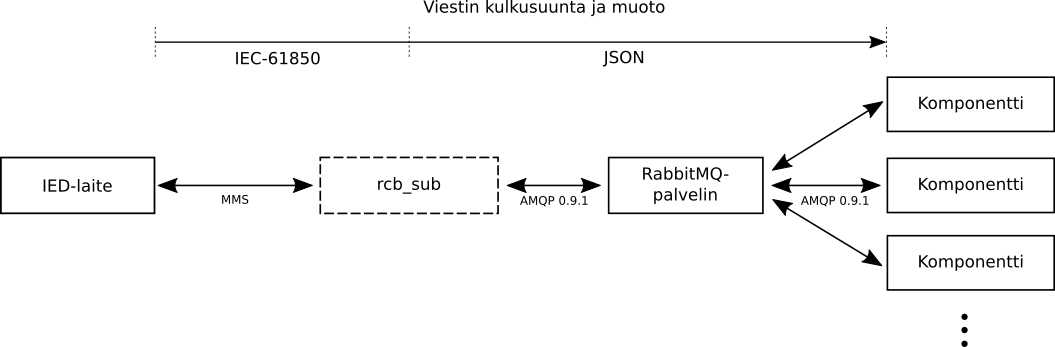
\includegraphics[width=1\textwidth]{pictures/planned-system-architecture.png}
	\caption{Suunnitellun järjestelmän arkkitehtuuri sekä viestin kulku ja muoto sen osapuolten läpi.}
	\label{fig:planned-system-architecture}
\end{figure}

AMQP-välittäjäpalvelin päädyttiin toteuttamaan RabbitMQ ohjelmistolla, joka on AMQP-stan\-dar\-diin perustuva välittäjäohjelmisto \cite{rabbitmq-homepage}. Väliohjelmistolle annettiin nimeksi rcb\_sub ja on merkitty kuvaan katkoviivalla. Nimeä käytetään tästä eteenpäin tekstissä viittaamaan kyseiseen komponenttiin. Kuvassa vasemmalla on IED-laite, josta rcb\_sub tilaa viestit MMS-protokollan avulla. Rcb\_sub prosessoi saapuneet viestit JSON-muotoon ja uudelleenjulkaisee ne RabbitMQ-palvelimelle. Järjestelmän muut komponentit tilaavat JSON-viestejä välittäjäpalvelimelta tarpeidensa mukaan.

Rcb\_sub päädyttiin toteuttamaan C-kielellä komentorivipohjaiseksi ohjelmistoksi. Tilauksen tekemiseen tarvittavat tiedot ohjelmalle annettiin komentoriviparametreinä. Rcb\_sub pystyi tilaamaan yhden IED-laitteen halutun määrän RCB-instansseja. AMQP-stan\-dar\-dis\-ta on olemassa eri versioita ja valittu RabbitMQ-ohjelmisto käytti versiota 0.9.1. Rcb\_sub käytti demosta tuttua libIEC61850-kirjastoa hoitamaan matalan tason IEC 61850 -stan\-dar\-din toiminnallisuuden.


\section{AMQP-välittäjäpalvelin}
AMQP-pohjaisen välittäjäpalvelimen toteutukseen löytyy erilaisia ohjelmistoja. Joita on mm. RabbitMQ, Apache Qpid ja StormMQ. Työssä AMQP-pohjaisen palvelimen toteuttamiseen valittiin RabbitMQ. RabbitMQ on ilmainen avoimen lähdekoodin välittäjäpalvelin ja sille on olemassa kattava tuki monelle eri kielelle asiakasohjelmiston toteuttamiseen \cite{rabbitmq-supported-languages}. Vertailun perusteella se vaikutti toteutukseen hyvältä vaihtoehdolta.

AMQP-standardista on julkaistu monta eri versiota, ja työn tekohetkellä viimeisin versio oli 1.0. RabbitMQ-ohjelmisto on suunniteltu käytettäväksi standardin version 0.9.1 kanssa, ilman asennettuja lisäosia. Versioiden välinen ero on suuri ja siirto uuteen ei ollut mahdollista, koska standardin versiot eivät olleet keskenään yhteensopivat. RabbitMQ tuki versiota 0.9.1 ja sen kehittäjät mieltävät standardin version 1.0 kokonaan eri protokollaksi \cite{RabbitMQ-Compatibility-and-Conformance}. Tämä ei kuitenkaan sen käyttöä haitannut, koska versio 0.9.1 kattaa kaikki suunnitellut hajautetun järjestelmän paradigmat. Paradigmoja olivat viestijono ja julkaisija-tilaaja. RabbitMQ:ta voi käyttää AMQP version 1.0 kanssa erillisellä lisäosalla. RabbitMQ lupaa jatkaa version 0.9.1 tukemista, jolloin sitä on myös mahdollista käyttää jatkossakin \cite{RabbitMQ-Compatibility-and-Conformance}.


\section{Tilauksen orkestrointi ja tiedon välitys}
Muun järjestelmän on tarkoitus ohjata rcb\_sub-ohjelman suoritusta. IED-laitteilta viestien tilauksia käyttäjä voi ohjata järjestelmän käyttöliittymästä. Tilauksen aloittaessa järjestelmä käynnistää rcb\_sub-ohjelmiston omana prosessinaan yhtä IED-laitetta kohti. Tilauksen loputtua järjestelmä lopettaa rcb\_sub-prosessin suorituksen. Suorituksen aikana tulevat virheet ohjataan järjestelmälle, joka voi toimia tarvittaessa niiden mukaan, esimerkiksi käynnistää prosessin uudestaan. Kaikkien rcb\_sub-prosessien on tarkoitus ohjata JSON-viestit saman RabbitMQ-palvelimen läpi muulle järjestelmälle.

Rcb\_sub-ohjelmaa oli tarkoitus ajaa prosessina, siispä se ei tarvinnut käyttöliittymää. Tämän takia se päätettiin toteuttaa komentorivipohjaisena ohjelmana. Muu järjestelmä oli rakennettu suoritettavaksi Linux-käyttöjärjestelmän päällä, joten rcb\_sub toteutettiin myös samalle käyttöjärjestelmälle. Jotta rcb\_sub voi tehdä tilauksen IED-laitteelle ja tietää mitkä RCB-instanssit tilataan, täytyy järjestelmän tarjota tämä tieto. Tarvittavaa tietoa ovat IED-laitteen ja AMQP-palvelimen IP-osoitteet, tilattavien RCB-instanssien viitteet ja arvot, viestien julkaisuun välittäjäpalvelimelle tarvittavat tiedot. RCB-instanssille kirjoitettavat arvot sisältävät vaihtoehtoiset kentät (OptFlds) ja liipaisimet (TrgOps). Julkaisuun tarvittavia tietoja ovat käytettävän \emph{vaihteen} (\emph{exchange}) nimi ja \emph{reititysavain} (\emph{routing key}). Vaihde on AMQP-palvelimella käsite, johon tilaajat tekevät tilauksia ja on vastuussa viestien reitittämisestä oikeille tilaajille. Reititysavain on viestin tunniste millä se julkaistaan. Tämän ja tilaajan tekemän tilauksen mukaan vaihde reitittää viestit oikeille tilaajille. Toisin sanoen reititysavain sisältää IED-laitteen tunnisteen. Tämän perusteella tilaaja voi tilata haluamansa IED-laitteen viestit.

Tiedon välittämiseen prosessien välillä on olemassa monia eri tapoja. Jos tieto on pysyvää ja siinä ei ole muutoksia, yksi vaihtoehto olisi ollut konfiguraatiotiedosto. Järjestelmässä kuitenkin tilattavien RCB-instanssien määrä ja IED-laitteen tiedot voivat muuttua. Tämän takia päädyttiin käynnistyksen yhteyteen annettuihin komentoriviparametreihin. Muu järjestelmän osa, joka rcb\_sub-prosessin käynnistää, voi kaiken tarvittavan tiedon antaa prosessille parametreillä käynnistyksen yhteydessä. Vaikka tieto tilauksien välillä muuttuu, prosessi käynnistetään aina viimeisimmillä tiedoilla. Ohjelmalle ei ollut asetettu vaatimusta, että tietoja pystyisi muuttamaan tilauksen aikana. Jos tietoja tarvitsee muuttaa, lopetetaan edellinen tilaus ja käynnistetään uusi prosessi uusilla parametreilla. Sama periaate on myös järjestelmän käyttöliittymässä. Myöhemmin tulevaisuudessa tarpeen vaatiessa voidaan siirtyä dynaamisen tilauksen muutokseen, mutta tällä hetkellä sille ei ollut tarvetta.

AMQP ei tarjoa julkaisujen mainostukseen mahdollisuutta, kuten käsiteltiin julkaisija-tilaaja-paradigman yhteydessä \cite{AMQP-specification}. Järjestelmän komponenttien pitää saada tieto olemassa olevista julkaisijoista muulta järjestelmältä. Tämä tieto järjestelmässä siirretään komponenteille tietokannan kautta. Kuvassa \ref{fig:example-use-case} on esitetty käyttötapaus esimerkki, jossa mittaustietoa käyttävä komponentti tilaa viestejä ja lähettää sen käyttäjän selaimen käyttöliittymään web-sokettia pitkin \cite{websocket}. Selaimessa JavaScript-koodi päivittää käyttöliittymän komponentteja saadun tiedon mukaan.

\begin{figure}[ht!]
	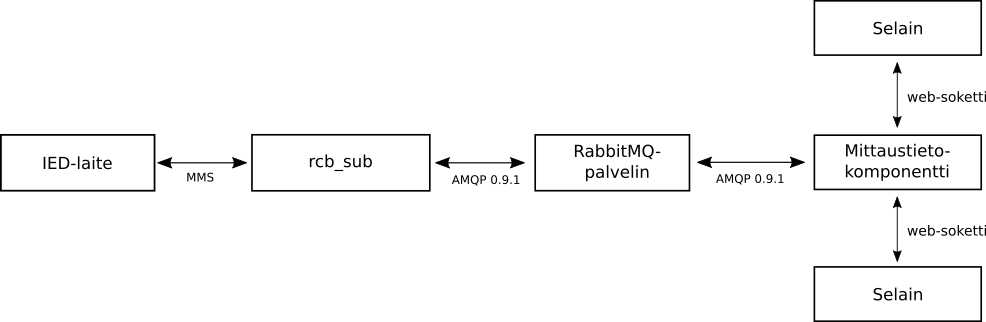
\includegraphics[width=1\textwidth]{pictures/example-use-case.png}
	\caption{Esimerkkikäyttötapaus, jossa mittaustietoa tilaava komponentti lähettää tietoa selaimen käyttöliittymään web-soketin avulla.}
	\label{fig:example-use-case}
\end{figure}


\section{Suorituskyky ja kielen valinta}
Ennen koko ohjelman uudelleenkirjoitusta, kokeiltiin demoa korjata vaihtamalla Ruby-tulkkia. Ruby:n oletustulkki yritettiin vaihtaa \emph{JRuby}-tulkkiin \cite{jruby-homepage}. Tavoitteena vaihdossa oli saada Ruby-ohjelma toimimaan ilman globaalia tulkkilukitusta (GIL). JRuby on Ruby-tulkki, joka suorittaa Ruby-koodia \emph{Java-virtuaalikoneen} (\emph{Java Virtual Machine}, lyhennetään \emph{JVM}) päällä. JRuby mahdollistaa säikeiden suorituksen rinnakkain JVM:n omilla säikeillä ja näin ollen suorituksen pitäisi olla nopeampaa \mbox{\cite{Youssef2013}}. Aidolla rinnakkaisuudella ohjelman suoritus ei olisi pysähtynyt viestin saapuessa takaisinkutsufunktion suorituksen ajaksi. Tämä ei vielä olisi kuitenkaan ratkaissut kaikkia ohjelmassa olevia ongelmia, kuten muistivuotoa ja hitaampaa suorituskykyä verrattuna käännettävään kieleen. Tämä toteutus ei kuitenkaan toiminut, ja yrityksen jälkeen päätettiin palata suunnitelmaan kirjoittaa koko ohjelma uudestaan. JRuby ei tukenut kaikkia projektin käyttämiä kirjastoja. Seurauksena olisi ollut saman projektin ylläpitäminen kahdelle eri tulkille tai asennettavien kirjastojen erottaminen. Kaikkiaan oli helpompaa kirjoittaa ohjelma alusta toisella tekniikalla.

Uuden toteutuksen kieleksi valittiin C-kieli. Isona syynä kielen valintaan oli sen suorituskyky. C-koodi käännetään alustalle suoraan konekäskyiksi, joiden suoritus on nopeampaa kuin tulkattavan kielen, kuten Ruby ja Python. Valintaan vaikutti myös tekijän iso mieltymys matalan tason ohjelmointiin ja C-kieleen. Kielen valinnan yhteydessä varmistettiin kaikkien suunniteltujen liitosten mahdollisuus. C-kielelle löytyi kirjastoja RabbitMQ-välittäjäpalvelimen käyttämiseen ja lisäksi JSON-rakenteen muodostamiseen. Hyötynä vielä C-kielen valinnasta oli, että demossa käytettyä libIEC61850-kirjastoa pystyttiin käyttämään suoraan ilman erillistä liitosta, koska kirjasto oli myös toteutettu C-kielellä.


\section{JSON-viestin rakenne}
IED-laitteelta saapuva viesti päädyttiin muuntamaan JSON-muotoon helpompaa luettavuutta varten. LibIEC61850-kirjastossa viestin tiedot esitetään ClientReport-struk\-tuu\-rin instanssina. Sen sisältöä voi lukea käyttämällä kirjaston tarjoamia funktioita \cite{libIEC61850-doc}.  Liitteessä \ref{ch:report-json-format} on esitetty JSON-viestin rakenne. JSON:n noudattaa pääosin standardin mukaista viestin rakennetta. Standardin määrittämä viestin rakennetta ja sisältöä käytiin läpi kappaleessa \ref{ch:viestin-rakenne}. Erona standardin malliin on, että rcb\_sub lisäsi jokaiseen attribuuttiin sen koko viitteen, tyypin ja koon bitteinä. Nämä tiedot todettiin tarpeellisiksi, koska niiden avulla tilaajan on helpompi ymmärtää viestin sisältö. Tarvittavat lisätiedot luetaan IED-laitteelta erillisellä palvelukutsulla ennen tilauksen aloittamista. Nämä tiedot yhdistetään saapuneen viestin kanssa ja sijoitetaan JSON-rakenteeseen. Tulevassa tekstissä käydään läpi JSON:in rakennetta ylhäältä alaspäin ja viitataan liitteen \ref{ch:report-json-format} rivinumeroihin.

JSON:in päätaso sisältää standardin mukaista viestin informaatiota riveillä 2--6. Viestin kenttien määrää pystyi muuttamaan RCB-instanssin OptFlds-attribuutilla. JSON:iin kuitenkin haluttiin lisätä kaikki mahdolliset kentät selkeyden vuoksi. Jos kenttä puuttui viestistä, asetettiin sen arvoksi JSON:issa \emph{null}-arvo. Esimerkiksi kentän \emph{confRevision} arvo rivillä 4 on \emph{null}. Tällöin RCB-instanssissa \emph{OptFlds}-attribuutin \emph{conf-revision}-bitti on ollut epätosi. Samaa periaatetta käytettiin kaikille muillekin vaihtoehtoisille kentille. Tällä periaatteella viestin \emph{OptFlds}-kentän arvo voitiin kokonaan jättää pois JSON:ista.

JSON-rakenne koostuu kahdesta sisäkkäisestä \emph{values}-taulukosta (alkavat riveiltä 7 ja 13). Ensimmäinen \emph{values}-taulukko riveillä 7--90 sisältää viestissä olevat datajoukon FCD- tai FCDA-viitteet ja niihin liittyvät kentät. Samalla periaatteella, kuin standardin määrittämässä viestin rakenteessa taulukon arvot 1--n:ään (kuva \ref{fig:iec61850-report-format}). Eli viestin \emph{Reason Code} arvo on laitettu \emph{reasonForInclusion}-attribuuttiin. Viestin \emph{DataRef}-kenttä on pilkottu kolmeen eri kenttään \emph{mmsReference}, \emph{reference} ja \emph{functionalConstraint}. Viestien viitteet tulevat MMS-protokollamäärityksen muodossa, eli pisteet (.) on korvattu dollarin merkillä (\$) ja viite sisältää funktionaalisen rajoitteen. Nyt \emph{mmsReference} sisältää viestin alkuperäisen MMS-viitteen, \emph{reference} sisältää standardin abstraktin viitteen ja \emph{functionalConstraint} sisältää funktionaalisen rajoitteen. Nämä on erotettu selkeyden takia, koska mahdollisesti jotkin komponentit saattavat tarvita standardin käyttämää abstraktia viitettä ja näin välttää tekstimuunnokset.

JSON:in sisempi \emph{values}-taulukko riveillä 13--31 sisältää FCA- tai FCDA-viitteen viitatut attribuutit. Jokaiseen attribuuttiin lisättiin sen koko viite, tyyppi ja koko bitteinä. Viitteen avulla tilaaja voi yhdistää arvon attribuuttiin ilman tietoa IED-laitteen hierarkiasta. Standardin määrittämässä viestissä saapuva viite on datajoukon FCD- tai FCDA-viittaus ja sen alla taulukko pelkkiä arvoja. Taulukon arvot ovat hierarkiassa oikeasti viitattujen attribuuttien arvoja. Standardin viestin ymmärtämiseen tilaaja tarvitsee lisätietoa IED-laitteen hierarkiasta, jotta arvo voidaan yhdistää oikeaan attribuuttiin. Lisäämällä tiedot viestiin helpotetaan järjestelmän komponenttien kehitystä ja arvojen lukua. Esimerkiksi riveillä 20--24 attribuutti LD0\_CTRL/CBCILO1.EnaCls.q, joka on tyyppiä \emph{bit-string}, on 13-bittiä pitkä ja sen arvo on 0. Standardin mukainen viesti sisältää vain arvon 0 ja siihen viittaavaan FCDA-viitteen LD0\_CTRL/CBCILO1.EnaCls. Standardin viestin pohjalta tilaajan täytyy katsoa arvon indeksi viestistä. Indeksillä tietää IED-laitteen hierarkiassa viitteestä LD0\_CTRL/CBCILO1.EnaCls alaspäin viitattu attribuutti. Standardin mukainen ratkaisu on vaikea ja ei sovi tarkoituksiin.

Lisätyt kentät sisältävät joitakin poikkeuksia. Kokoa bitteinä ei ole lisätty \emph{boolean} ja \emph{utc-time} tyyppisille attribuuteille, koska tätä tietoa ei saa IED-laitteelta. \emph{Bit-string} tyypille lisättiin kaksi arvo-kenttää \emph{valueLittleEndian} ja \emph{valueBigEndian} yhden sijaan, koska se on mahdollista lukea eri bittijärjestyksellä (little ja big endian). Aikayksiköt päätettiin antaa suoraan samassa formaatissa kuin viestissä. Viestin päätason aikaleima on millisekunteja \emph{UNIX}-ajanlaskun alusta 1. tammikuuta 1970 klo 00:00:00 UTC (epoch) tähän hetkeen. Attribuuteissa tyypiltään \emph{utc-time}, luku on sekunteja samasta UNIX-ajanlaskusta tähän hetkeen \mbox{\cite[s.~26--27]{IEC61850-7-2}}.